% Put labels, etc., on figures using PSTricks.
% Use dvips -E <file>.dvi -o <file>.eps to create encapsulated PostScript.
%
\documentclass[12pt]{article}
\usepackage{graphicx}
\usepackage{pstricks}
\pagestyle{empty}

\begin{document}
\rput(5,-5){
\rput(.1,-.1){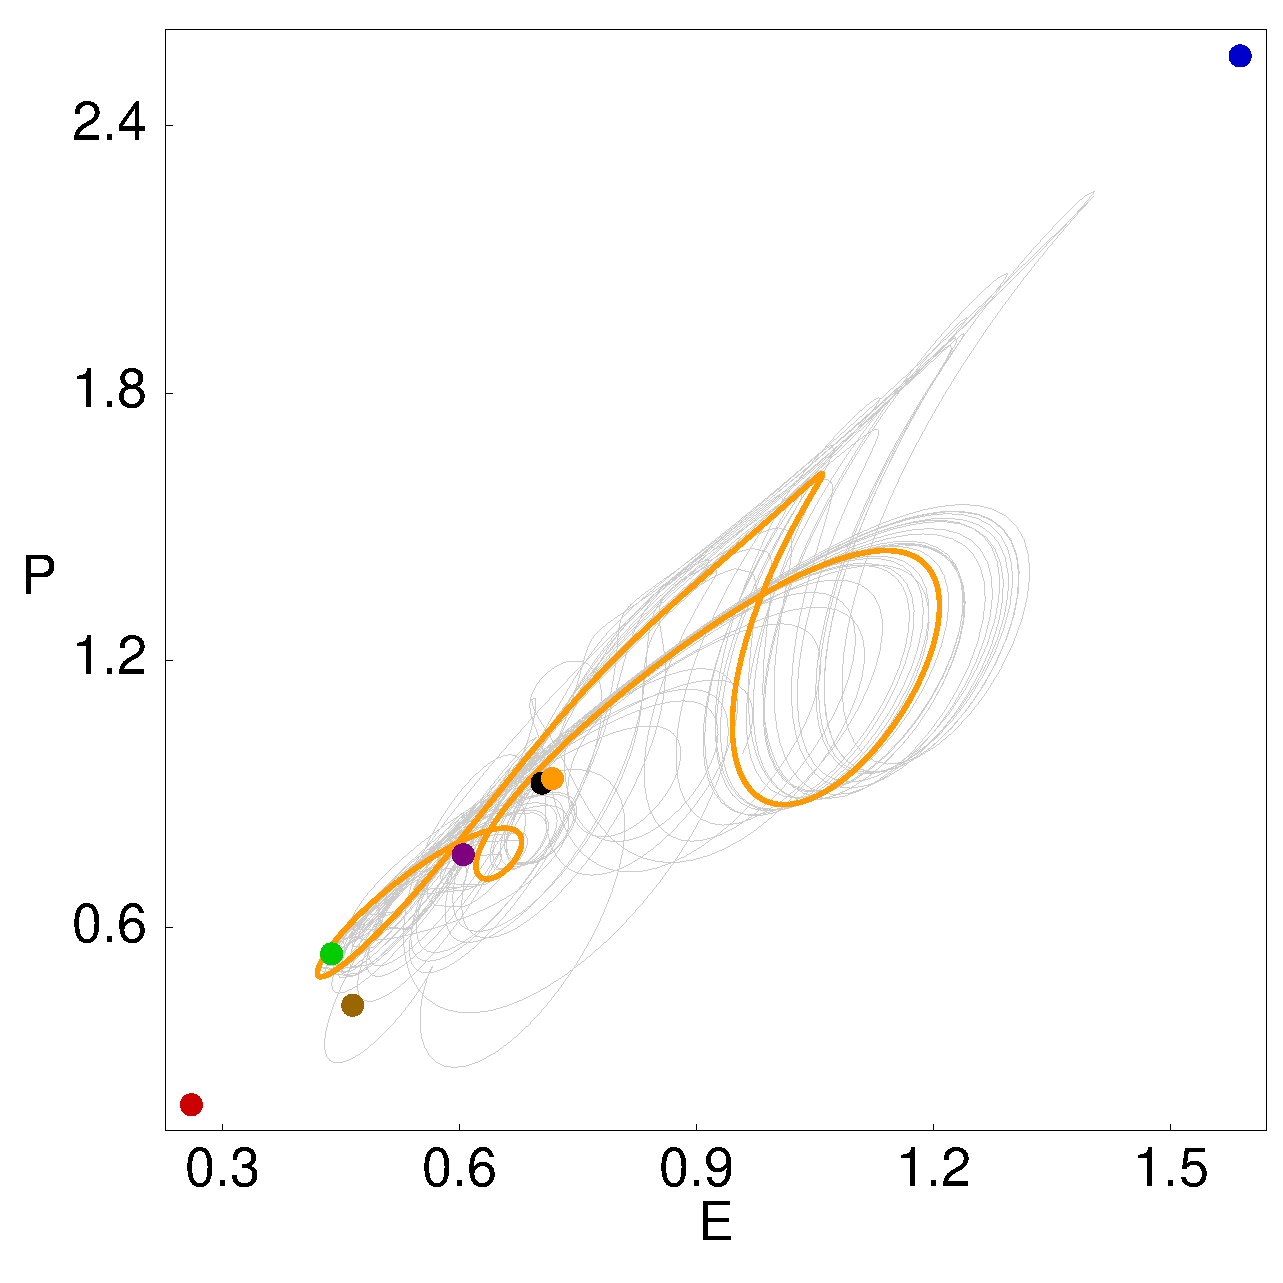
\includegraphics{../../rpo_ks/figs_pst/equivaEP.eps}}

\huge

\psframe*[linecolor=white](-6.5,6)(-5.5,7)
\psframe*[linecolor=white](6,-6.5)(7.2,-5.5)

\rput(9.2,9.3){E$_3$} \rput(-6.8,-7.4){E$_1$}

\psline[linewidth=2pt]{->}(-6.5,-4.5)(-5.2,-5.35)\rput(-7,-4.4){E$_2$}
\psline[linewidth=2pt]{->}(0.2,-7.2)(-4.7,-6.3)\rput(1.5,-7.3){TW$_{\pm1}$}
\psline[linewidth=2pt]{->}(-5.3,-2.7)(-3.05,-3.7)\rput(-6,-2.2){TW$_{\pm2}$}
\psline[linewidth=2pt]{->}(0,6.5)(3.7,3.7)\rput(0,7){``Turbulence''}
\psline[linewidth=2pt]{->}(4,-5.5)(3.2,-2.7)\rput(7,-5.5){$T_p\simeq 33\,,\ell_p\simeq 11$}
\psline[linewidth=2pt]{->}(-2,2.5)(-1.45,-2.3)\rput(-3,4){$T_p\simeq 33\,, \ell_p\simeq 11$,}\rput(-3,3){Time Average}
\psline[linewidth=2pt]{->}(-5,0)(-1.65,-2.4)\rput(-5,1.5){``Turbulence'',}\rput(-5.,0.5){Time Average}


% Use grid command below to place objects at specified coordinates.
% \psgrid[subgriddiv=1,griddots=10](-8,-8)(10,10)
}
\end{document}
